

\chapter{Datenaufbereitung} \label{prepareData}

Um die Deformation im eingespannten Zustand zu erkennen, muss das komplette Werkstück
als digitales Modell existieren, um es mit anderen Modellen vergleichen zu können.
Das hier zu entwickelnde Verfahren soll die Deformation nur in einer zweidimensionalen Perspektive erkennen. 
Das ist weniger komplex, hat aber zur Folge, dass Bauteile mit unterschiedlichen 
Oberflächenhöhen nicht vollständig analysiert werden können. 
Geometrie und Oberflächeninformationen des eingespannten Bauteils liegen 
in Form von mehreren Pointclouds vor.
Diese Daten wurden mithilfe eines Laser-Profilsensors aufgenommen 
(siehe Kapitel \ref{lasers}). Durch diesen Prozess 
entstehen Messfehler und Ausreißer. Diese Punkte verfälschen das Verfahren da sie 
nicht auf dem eingespannte Bauteil liegen. Die Genauigkeit des Verfahrens profitiert, 
wenn diese Punkte entfernt werden. Ausreißer sind in Abbildung \ref{fig:pcs} (a) 
zu sehen.

\section{Pointcloud filtern}
    
Ausreißer können aus Pointclouds entfernt werden, indem einzelne Punkte 
relativ zu ihren Nachbarpunkten im dreidimensionalen Raum betrachtet werden.
Zur Erkennung und Entfernung von Ausreißern sind in der Open-Source
Bibliothek 'Open3D' zwei Methoden vorhanden. 
Die Methode \glqq radius\_outlier\_removal\grqq~entfernt Ausreißer basierend auf 
einem konfigurierbaren Radius. Punkte die weniger als n andere Punkte in dem Radius 
haben werden entfernt. Die andere Methode lautet 
\glqq statistical\_outlier\_removal\grqq~ 
und entfernt alle Punkte, die weiter von ihren Nachbarn entfernt sind, als die 
statistische Varianz aller Entfernungen. \cite{Zhou.30012018}

Die erste Methode eignet sich gut, wenn die Maße des Objekts bekannt
sind. Dann kann der Radius entsprechend der Größenordnung des Bauteils gewählt werden.
Da das hier zu entwickelnde Verfahren sich nicht auf eine Bauteilgeometrie 
beschränken soll, ist dieses Verfahren nicht geeignet. 
Durch eine Annahme des Radius würden ein Bias 
zu kleinen oder großen Bauteile entstehen.
Stattdessen wird die statistische Herangehensweise genutzt. 
Hier werden Punkte gelöscht, die weiter von ihren benachbarten Punkten entfernt
sind als der durchschnittliche Abstand der Punkte in der gesamten Pointcloud. 
Umso mehr benachbarte Punkte betrachtet werden, desto länger dauert der Filterprozess.

Beim Filtern werden zwischen sieben und zehn Prozent der Punkt in der Pointcloud entfernt.
In Abbildung~\ref{fig:pcs} sind Pointclouds vor und nach dem Entfernen von Ausreißern 
dargestellt.

\begin{figure}[H]
    \centering
    \begin{minipage}{0.45\textwidth}
        \centering
        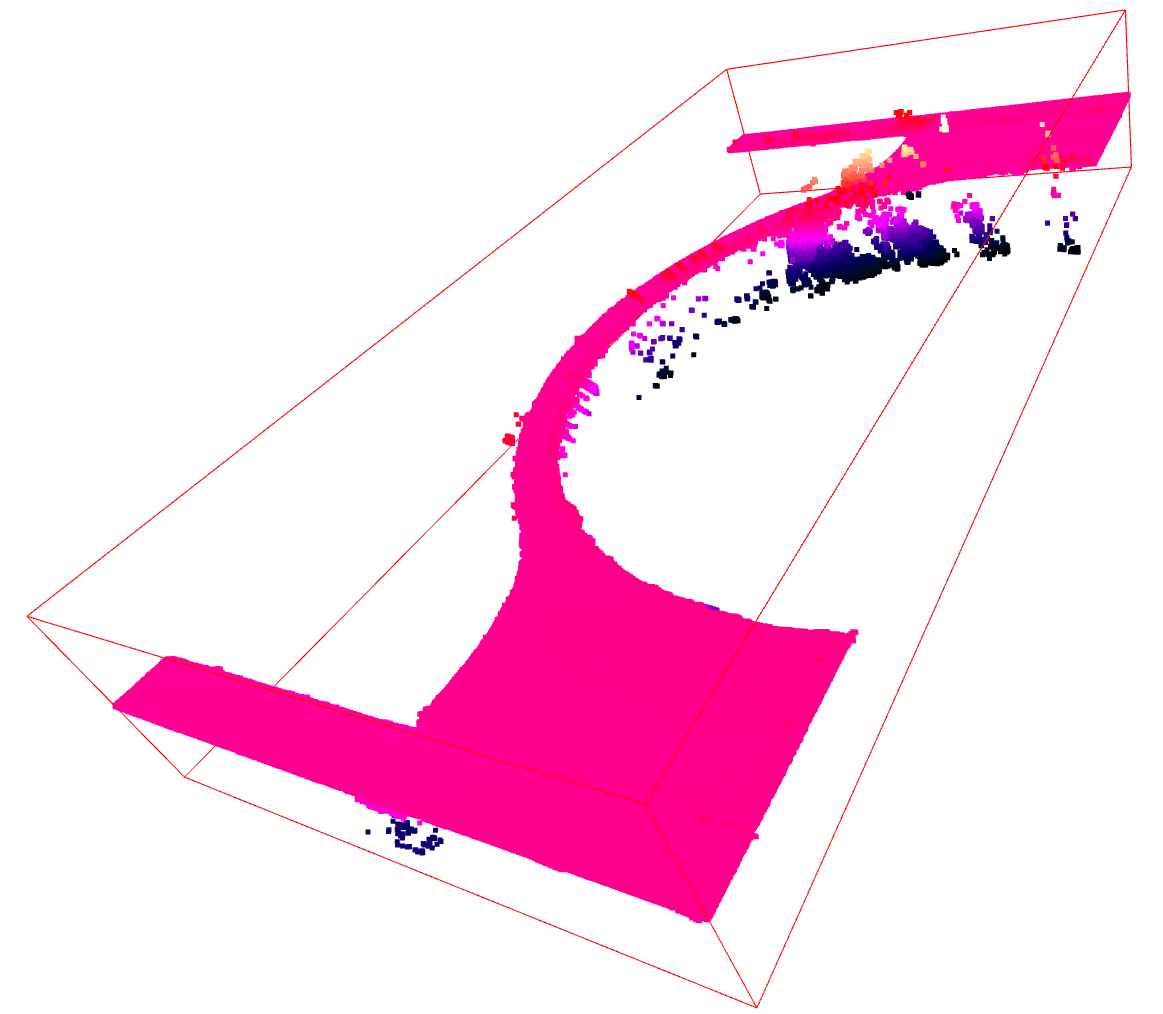
\includegraphics[width=\textwidth]{images/pc_with_outliers.PNG} % first figure itself
        \caption*{(a)}
    \end{minipage}\hfill
    \begin{minipage}{0.45\textwidth}
        \centering
        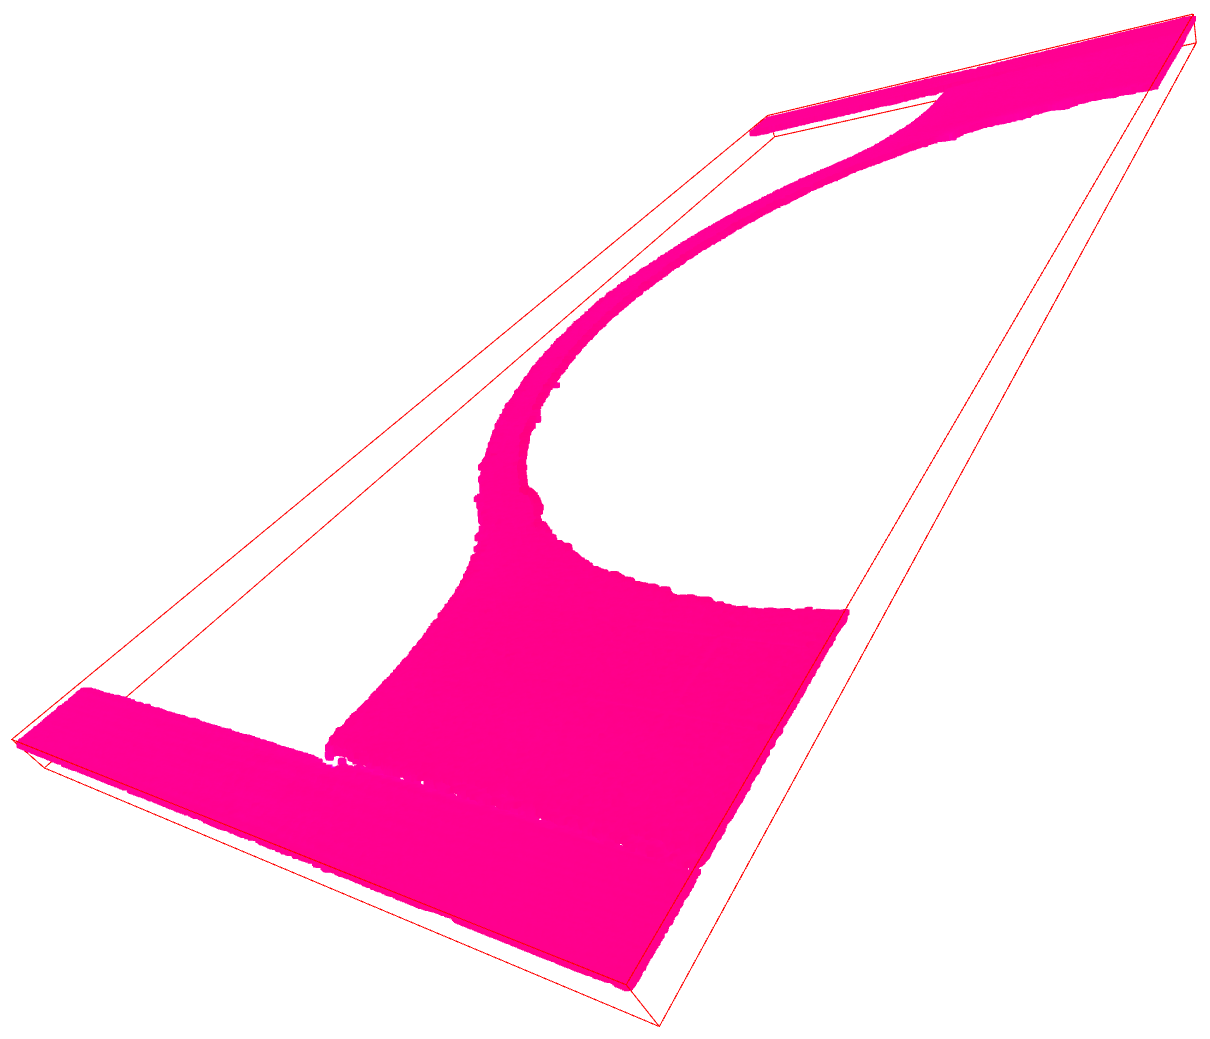
\includegraphics[width=\textwidth]{images/pc_without_outliers.PNG} % second figure itself
        \caption*{(b)}
    \end{minipage}
    \caption{Pointcloud eines Metallbauteils, in (a) ohne Filterung,
    in (b) mit den Ausreißern entfernt.}
    \label{fig:pcs}
\end{figure}

\section{Pointcloud in Bild konvertieren}

Um Rechenzeit zu sparen und die zahlreichen Funktionen bereits bestehender
Bilderkennungsbibliotheken nutzen zu können, werden die Pointclouds in Bilder 
konvertiert. Hierfür wird zunächst ein leeres Bild mit den gleichen 
Maßen der Pointcloud erstellt. Anschließend wird über alle Punkte der
Pointcloud iteriert und der Pixel an den 
entsprechenden X- und Y-Koordinaten des Punktes auf einen Helligkeitswert gesetzt.

Um Rechenzeit und Speicherkapazitäten zu schonen und 
da es für die Berechnungen ausreichend ist, wurden 
8-Bit-Single-Channel-Bilder verwendet, die nur Helligkeitswerte abbilden und keine 
Farbinformationen.
In diesen Bildern kann jeder Pixel einen Wert zwischen 0 und 255 annehmen. 
Der entsprechende Helligkeitswert wird wie folgt berechnet:
\begin{align*}\label{calc:brightness}
    value_p = \frac{Z - min_z}{max_z - min_z} \cdot (max_{brightness} - min_{brightness}) + min_{brightness}
\end{align*}
Der resultierende Wert ist die Helligkeit, die dem Pixel zugewiesen wird.
$Z$ ist die Z-Koordinate des Punktes in der Pointcloud. $min_y$ und $max_y$ sind 
die Grenzen der Z-Koordinate, diese werden gebraucht um die Helligkeit relativ 
zu der Höhe zu berechnen. $min_{brightness}$ und $max_{brightness}$ sind die gewünschten Grenzen der 
Helligkeit. In unserem Fall sind $min_{brightness} = 0$ und $max_{brightness} = 255$ da ein acht Bit Bild
verwendet wird.

In Abbildung \ref{fig:image_from_pc} ist das resultierende Bild eines Scans von einem 
FDM Bauteil zu sehen. Es fällt auf, dass kaum Helligkeitsveränderungen
im Bild sichtbar sind. Das liegt an derselben Problematik, an der der ICP-Algorithmus
 (vgl. Kapitel \ref{icp}) häufig
scheitert. Reale Datensets spiegeln die Realität nicht ganzheitlich korrekt wider, 
sondern beinhalten Messfehler und Streuungen, die trotz der Filterung der Pointcloud
bestehen bleiben.

\begin{figure}[H]
    \centering
    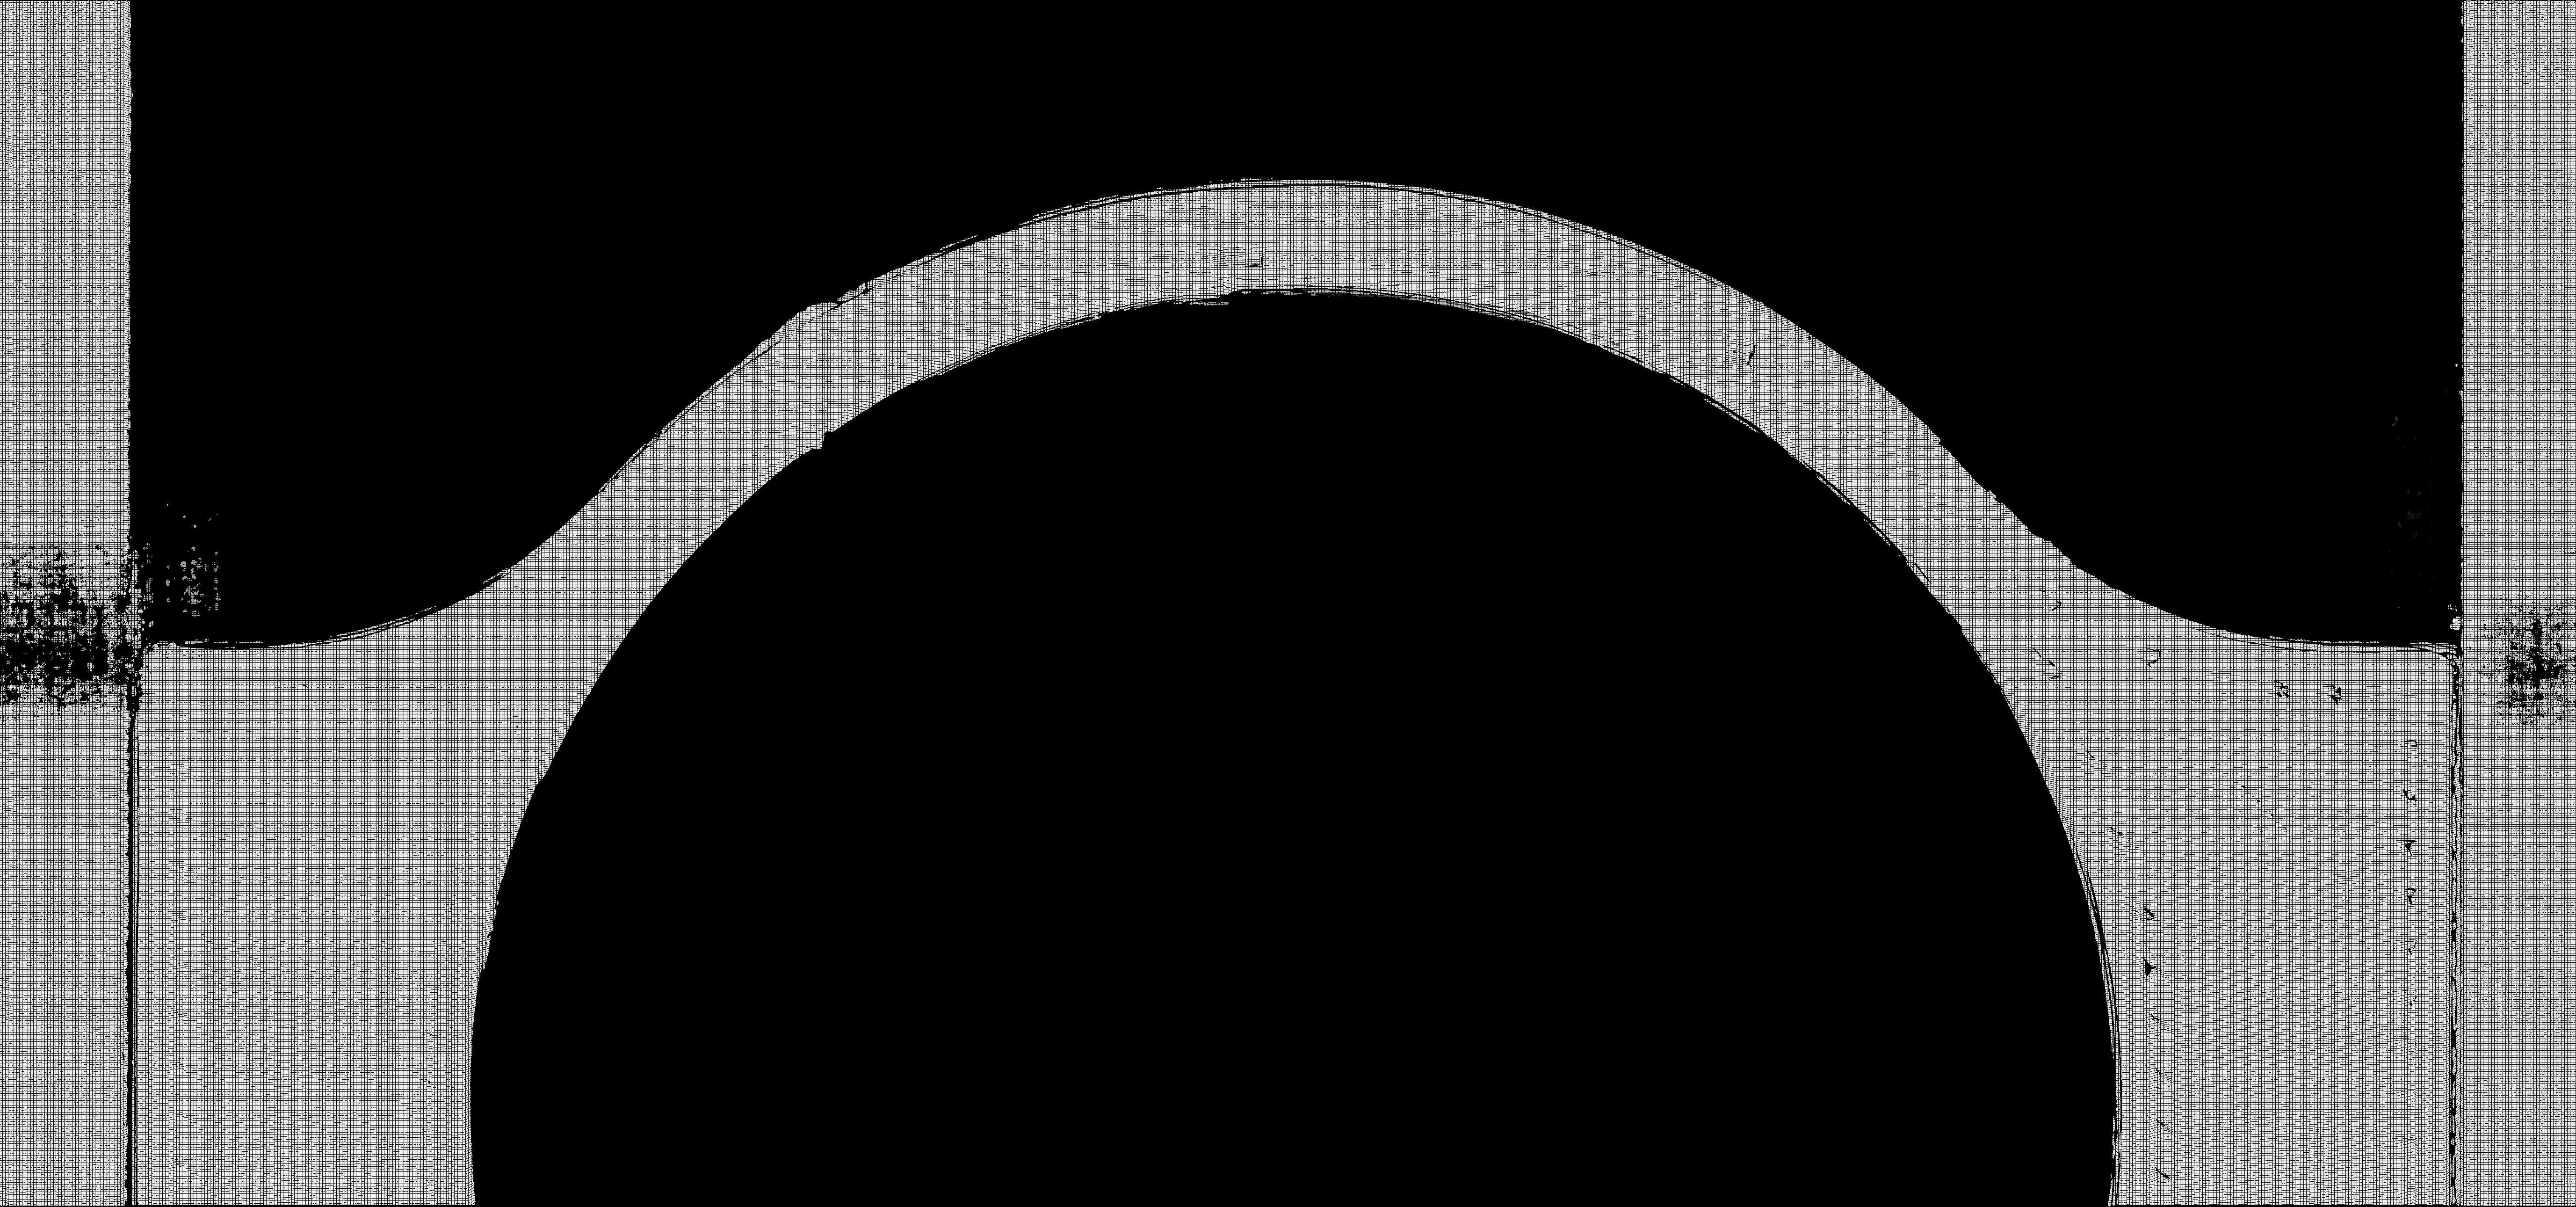
\includegraphics[width=0.9\textwidth]{images/fdm_top_100p.png}
    \caption{Resultat der Pointcloud zu Bild Konvertierung eines FDM Bauteils, 
    ohne zusätzliche Filterung der Höheninformationen.}
    \label{fig:image_from_pc}
\end{figure}

Damit das resultierende Bild die Höheninformationen besser widerspiegelt, werden 
die Scandaten erneut gefiltert. In diesem Filterprozess werden die Daten nicht, 
wie zuvor, im dreidimensionalen Raum betrachtet, sondern es werden ausschließlich 
die Höheninformationen der Pointcloud betrachtet.

Abbildung \ref*{fig:brightness} zeigt die Häufigkeitsverteilung der Höhenwerte einer
Pointcloud von dem Demonstratorbauteil (siehe Kapitel \ref{demo_Bauteil}). 
In blau ist die Verteilung der Punkte auf 
einem Demonstratorbauteil zu sehen, das aus Metall gedruckt wurde, orange zeigt die 
Verteilung der Punkte auf einem Kunststoffteil.
In dem oberen Histogramm 
sind die Häufigkeiten der Höhenwerte zu sehen. Der Datensatz wurde in 1000 gleich große
Teile gruppiert, jeder Balken repräsentiert eine Gruppe.
In \ref*{fig:brightness} (b) ist das Histogramm mit dem gleichen Datensatz wie in (a) 
dargestellt, aber mit der y-Achse 
logarithmisch skaliert um kleine Prozente deutlich zu machen die in Diagramm
(a) nur schwer oder gar nicht sichtbar sind. 
Die meisten Höhenwerte treten bei ca. 80 mm beziehungsweise 85 mm auf, 
sie gehören zu den Punkten, die auf dem Demonstratorbauteil liegen, 
es treten allerdings auch Werte darunter und darüber auf. 
Die in \ref*{calc:brightness} vorgestellte Formel benutzt allerdings 
die absoluten Minimum und Maximum Werte.
Alle Punkte die tatsächlich auf dem Bauteil werden also entsprechend wenig
berücksichtigt. Dies kann verhindert werden, indem Werte, die weniger häufig 
auftreten, entfernt werden.

\begin{figure}[H]
    \centering
    \begin{minipage}{\textwidth}
        \centering
        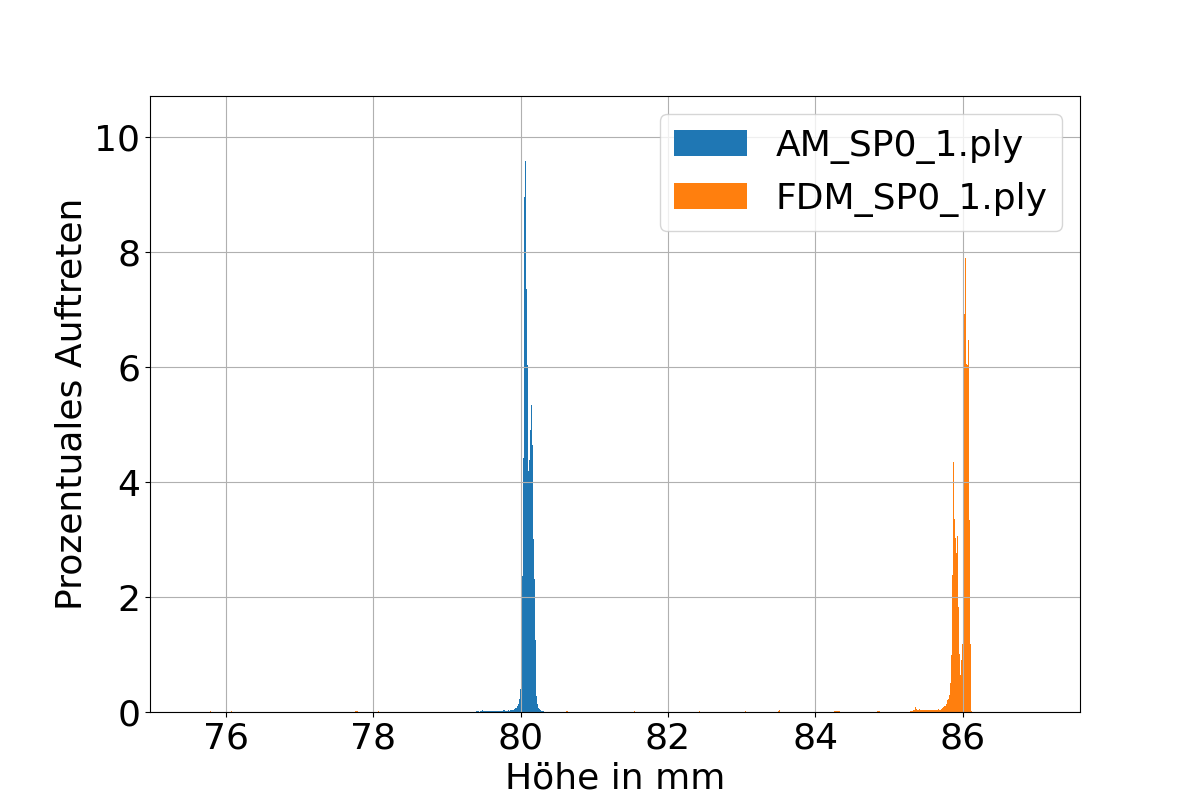
\includegraphics[width=0.8\textwidth]{images/height_occurange.png} % first figure itself
        \caption*{(a)}
    \end{minipage}\hfill
    \begin{minipage}{\textwidth}
        \centering
        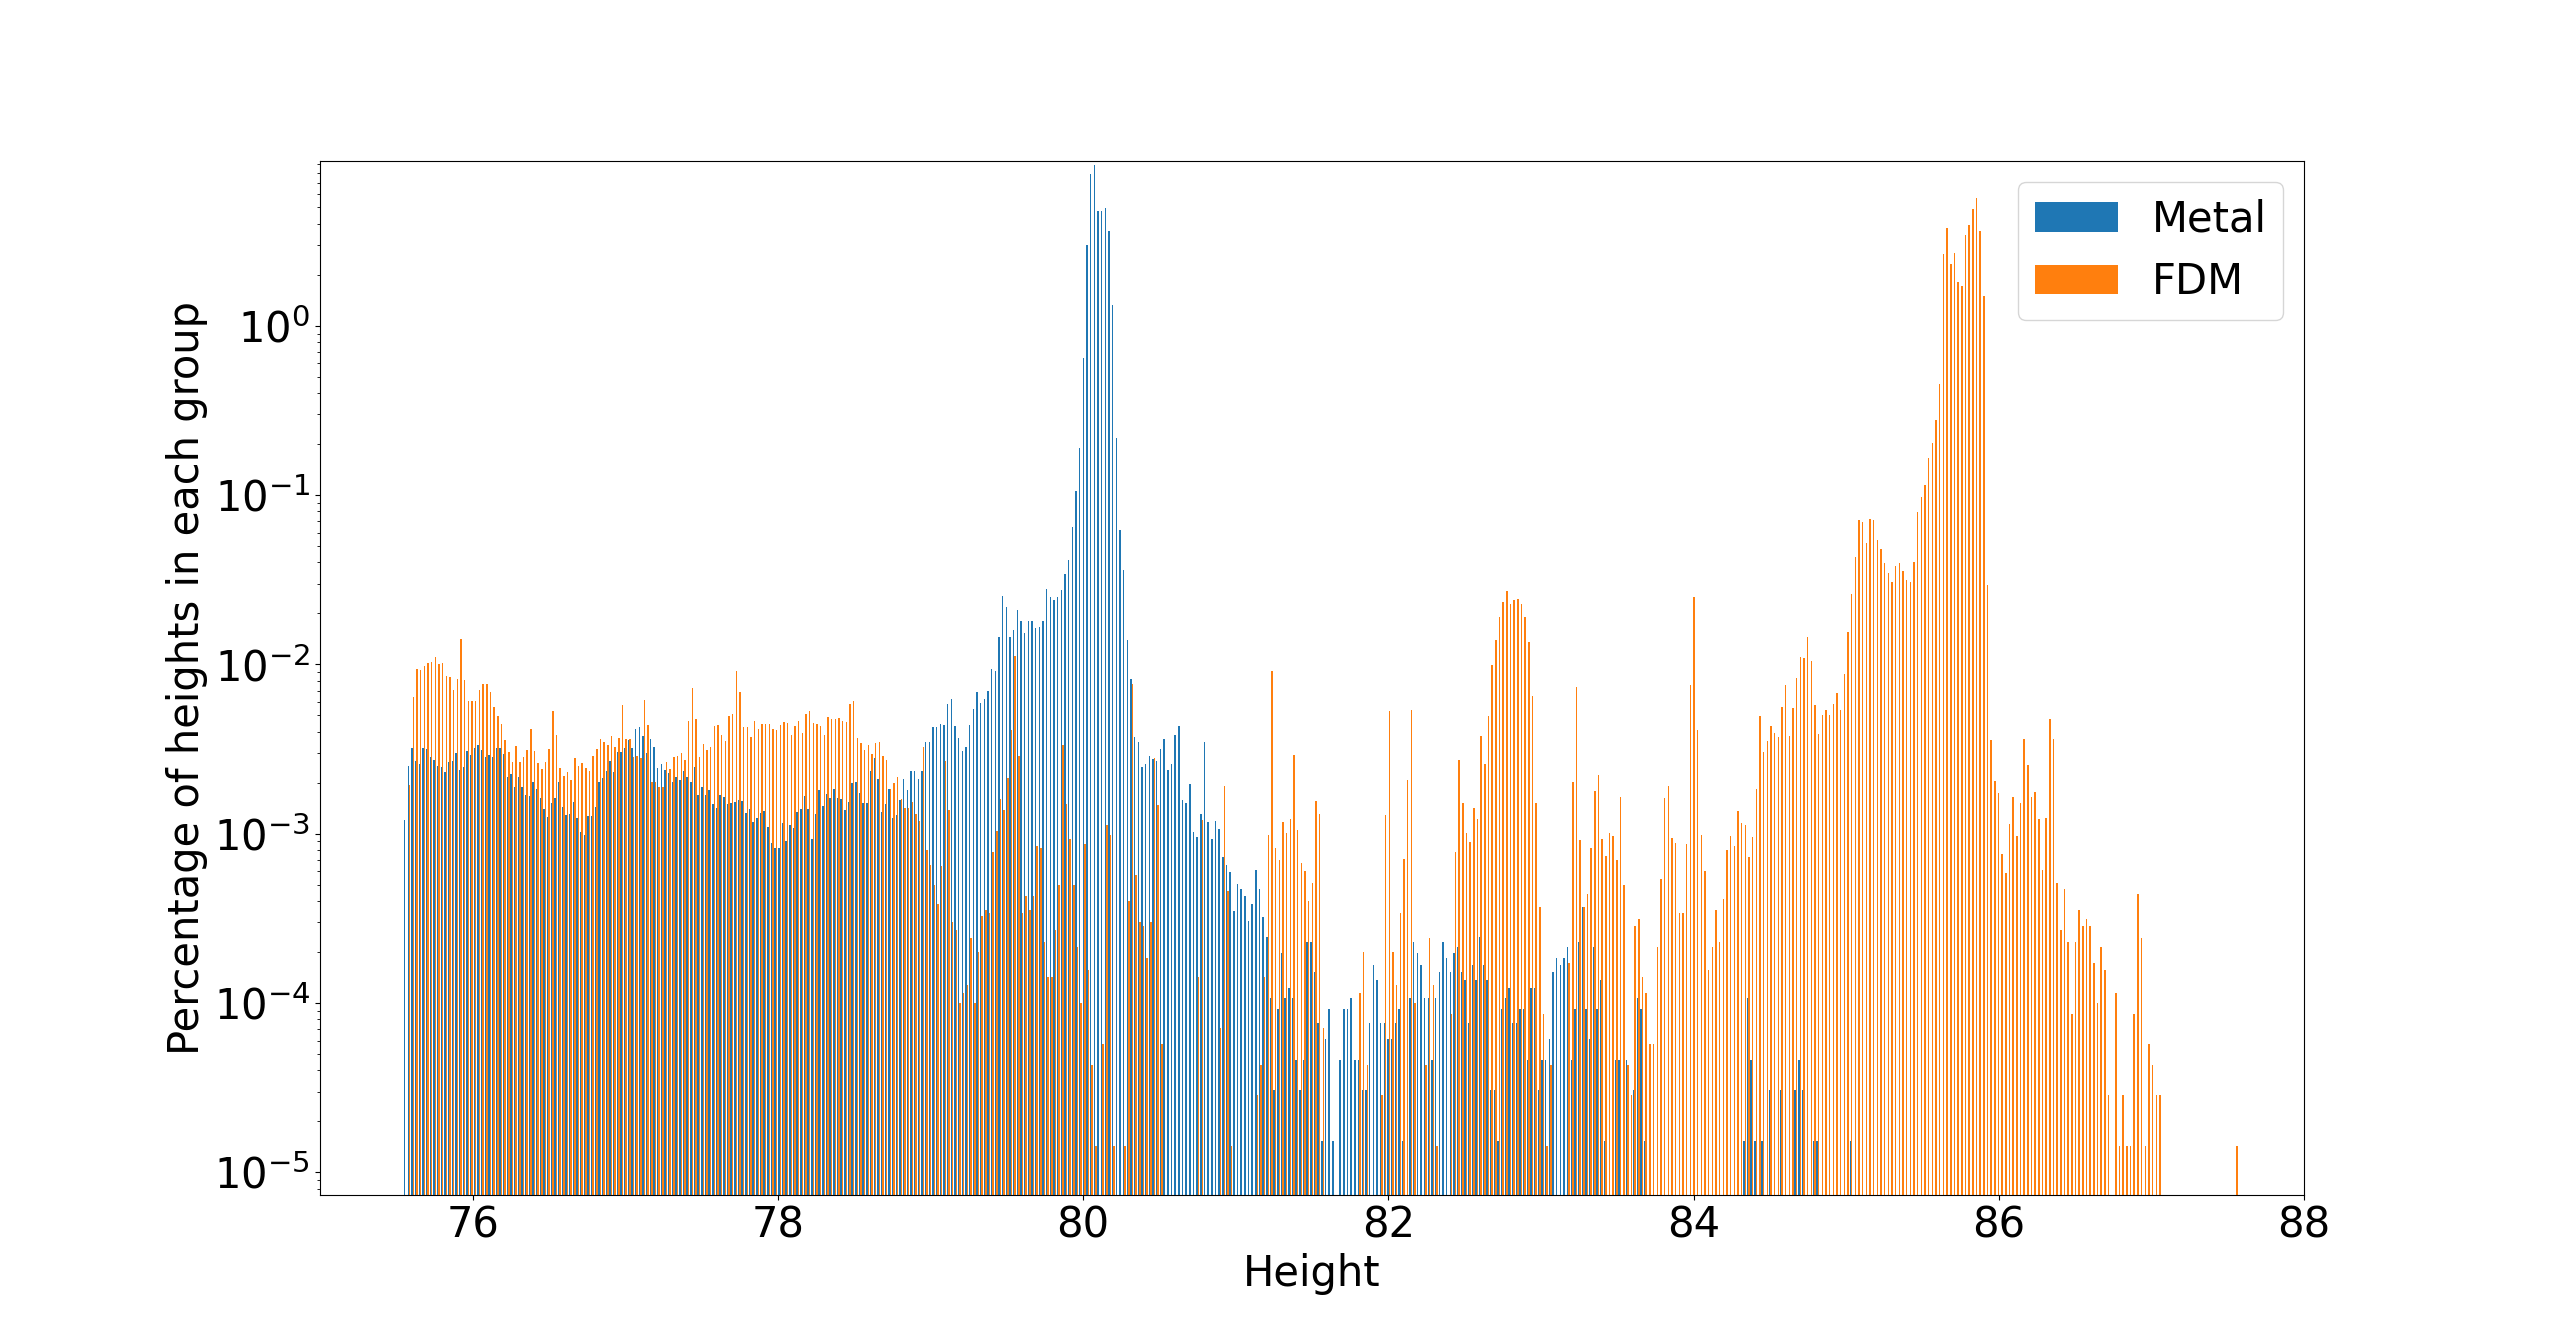
\includegraphics[width=0.8\textwidth]{images/height_occurange_log.png} % second figure itself
        \caption*{(b)}
    \end{minipage}
    \caption{Auftreten der Höhenwerte in den Scandaten der Demonstratorbauteile. 
    (a): Das Histogramm ist nicht skaliert. (b): Logarithmische Skalierung der 
    Höheninformationen. Hier ist zu sehen, dass die Höhenhäufigkeiten streuen.}
    \label{fig:brightness}
\end{figure}

Werden alle Höhenwerte nach der Häufigkeit ihres 
Auftretens in der Pointcloud sortiert, und der n-ten Prozentsatz entfernt, können
zusätzliche Ausreißer entfernt werden.
Ränder und Oberflächenstrukturen auf dem Bauteil können dadurch deutlich besser erkannt werden. 
Dadurch sind auch die Markierungen auf der linken und rechten Seite sichtbar geworden,
diese sollen bei der Registrierung
helfen. Zusätzlich sind die Spuren und Lücken die durch den FDM 
Herstellungsprozess entstehen zu sehen.
Durch das Filtern der Höheninformationen sind Oberflächenstrukturen nicht nur besser
erkennbar, auch die Ränder treten genauer hervor. 
Dadurch können die Bilder im weiteren Schritt korrekt zusammengefügt werden.
In Abbildung \ref{fig:10p} ist das resultieren Bild zu sehen, wenn nur die zehn Prozent
häufigsten Höhenwerte verwendet werden.
Die Spuren des FDM Fertigungsprozess sind deutlich zu sehen.

\begin{figure}[H]
    \centering
    \includegraphics[width=0.95\textwidth]{images/fdm_top_10p.png}
    \caption{Resultat der Pointcloud zu Bild Konvertierung eines FDM Bauteils.}
    \label{fig:10p}
\end{figure}
